\documentclass[conference]{IEEEtran}
\IEEEoverridecommandlockouts
\usepackage{cite}
\usepackage{amsmath,amssymb}
\usepackage{graphicx}
\usepackage{booktabs}
\usepackage{multirow}
\usepackage{url}
\usepackage[hidelinks]{hyperref}
\usepackage{xcolor}

\begin{document}

\title{Semantic Retrieval of Aviation Safety Reports with Frozen Sentence Embeddings\\
\large Project Milestone (Phase 2)}

\author{\IEEEauthorblockN{Jacob Tang \qquad Aarambh Shrestha}
\IEEEauthorblockA{CIS 634 Natural Language Processing (Dr.\ Mansi Bhavsar)}}

\maketitle

\begin{abstract}
Safety analysts need to find past NASA ASRS reports that describe the same operational
problem as a new one, even when pilots word it differently. We built one pipeline that
indexes all 47,723 reports in a public ASRS release and scores keyword search (BM25),
frozen sentence encoders from 22M to 0.6B parameters, and rank-fusion hybrids on three
evaluation tracks. The first track uses 1,000 analyst synopses as paraphrase
queries. The second uses 40 analyst-style issue descriptions with graded relevance labels
derived from NASA's coding (``silver'' labels). The third is a 100-item test of whether
meaning-changing edits (negation, numbers, direction, event order) fool the models.
Contrary to our expectation, BM25 is the strongest single system at finding the report a
synopsis summarises (MRR@10 0.425 vs.\ 0.268 for MiniLM). Larger encoders narrow the gap
(best: Qwen3-Embedding-0.6B, 0.371), and only fusing Qwen3 with BM25 beats BM25 (0.446,
$p{=}0.018$). On topical queries Qwen3 is the only encoder to beat BM25 (nDCG@10 0.746 vs.\
0.630, $p<0.001$). A graph over NASA's anomaly codes would lift MRR@10 to 0.643 with
perfect query linking, but a learned linker gains only 0.010. When word
overlap is controlled, the best encoders tell a same-meaning sentence from a minimally
edited one 85--89\% of the time. Yet every system prefers the edited sentence when it
shares more words (at most 35\% correct), and event order stays near chance.
\end{abstract}

\section{Introduction}
The Aviation Safety Reporting System (ASRS) holds hundreds of thousands of voluntary,
free-text incident reports. Keyword search misses paraphrases (``climbed through our
assigned altitude'' vs.\ ``overshot the level-off''), while frequent words such as
``altitude'' return thousands of off-topic hits. Sentence-BERT-style encoders
\cite{reimers2019sbert} encode each passage once and compare by cosine, so they are fast
enough to search a whole archive. They are trained on general English, however, and can
blur details such as negation or event order that decide the meaning of a safety report
\cite{ettinger2020bert}. Our research question is: \emph{can a frozen sentence embedding
retrieve ASRS reports that describe the same issue when the wording differs, and does the
ranking fail under negation, number (e.g.\ altitude), direction or event-order changes?} By this
milestone the data pipeline, all four proposed systems, and an evaluation harness are
implemented, and we have first results on all three evaluation tracks.

\section{Approach}
\subsection{Retrieval systems}
\textbf{BM25} \cite{robertson2009bm25} ($k_1{=}1.2$, $b{=}0.75$, Lucene IDF) on
lowercased, stopword-filtered, Snowball-stemmed tokens. We implemented it on sparse
matrices so that the same corpus statistics can also score arbitrary sentence pairs for
the meaning-change test. A unit test checks that its scores equal those of the
\texttt{bm25s} library.
\textbf{Dense encoders} are used frozen through sentence-transformers.
all-MiniLM-L6-v2 \cite{wang2020minilm,minilmcard} (22M parameters, 384-d, trained on 1B
sentence pairs) and e5-small-v2 \cite{wang2022e5} (33M parameters, 384-d,
\texttt{query:}/\texttt{passage:} prefixes) produce L2-normalised vectors, and search is
exact (every chunk is scored).
Narratives are longer than the encoders' context windows, so we encode \emph{chunks} and
score a report $d$ by its best chunk (MaxP \cite{dai2019maxp}):
\begin{equation}
s(q,d)=\max_{c\in d}\cos\big(f(q),f(c)\big),
\end{equation}
returning $\arg\max_c$ as the matched passage shown to the analyst.
\textbf{Hybrids} fuse two report rankings with reciprocal rank fusion \cite{cormack2009rrf},
$s(d)=\sum_{r}1/(60+\mathrm{rank}_r(d))$, over the top 1,000 reports of each component.
\textbf{Taxonomy graph.} Graph-based retrieval (GraphRAG \cite{edge2024graphrag}) links
documents through shared entities, and ASRS already has such a graph: each report links to the anomaly codes NASA's analysts assigned to it (63 codes used at least
20 times; 2.6 per report). A classifier (TF-IDF, one-vs-rest logistic regression on train-split synopses)
links a query to the graph by predicting each code's probability, and we rerank BM25's
top 100 by
\begin{equation}
s(q,d)=z\big(\mathrm{BM25}(q,d)\big)+\lambda\,z\big(\log P(Y_d\mid q)\big),
\end{equation}
where $\log P(Y_d\mid q)$ is the log-likelihood of $d$'s code set under these
independent per-code probabilities and $z$ standardises over the 100 candidates. $\lambda$
is tuned on 1,000 held-out train-split synopses. An \emph{oracle} variant links the query
to the target report's own codes, which bounds what perfect linking could give.

\subsection{What is ours}
We wrote the data pipeline, the BM25 implementation, MaxP scoring and fusion, the
taxonomy-graph reranker, a config format in which adding a model takes one YAML entry,
the query set and its labeling rules, the meaning-change test set, and all evaluation
code (about 1,400 lines of Python, with 22 unit tests). We reuse sentence-transformers,
Hugging Face \texttt{datasets}, scikit-learn and PyStemmer, and the nine pretrained
checkpoints in Tables~\ref{tab:main} and~\ref{tab:ext}.

\section{Experiments}
\subsection{Data and pre-processing}
We use \texttt{elihoole/asrs-aviation-reports} \cite{hoole2023asrs}: 47,723 de-identified
reports (Jan.\ 2012--Mar.\ 2022) split into 38,655 train, 4,295 validation and 4,773 test.
Each record has one or two reporter narratives (319 words on average, 15.2M words in total), an
analyst synopsis (27 words), and NASA analyst codes. We search the narratives only.
Pre-processing went through two versions; the steps of the current one (v2) are:
\begin{enumerate}
\item \textbf{Comma repair.} The export replaced every comma with a semicolon
(``10;000~FT'', ``IAF; we set''). We restore commas in the free text so that numbers
and clauses read as normal English. The coded fields keep ``;'' as their list separator.
\item \textbf{Placeholder removal.} 2,906 second narratives (26\%) are editorial notes,
e.g.\ ``[Report narrative contained no additional information.]''. We drop them (see
\S\ref{sec:prep-finding}).
\item \textbf{Incident grouping.} Union-find over shared accession numbers and identical
narratives finds 70 reports that describe the same incident as another record; 13 such
groups cross the official splits. Retrieving a sibling report counts as correct, and the
planned fine-tuning will split by group.
\item \textbf{Chunking.} Narratives contain no paragraph breaks, so we pack sentences
into windows of at most 150 words with a one-sentence overlap. A leftover tail under 40
words is merged into the previous window (so a few windows reach 189 words). This gives 136,842 chunks (2.9 per report;
150 WordPiece tokens on average, 99th percentile 222), which fit MiniLM's 256-token limit.
\end{enumerate}

\subsection{Evaluation}
\textbf{Synopsis track (automatic).} The query is the analyst's synopsis of one of 1,000
validation-split reports (seed 13). Analysts write the synopsis after reading the
narrative, so it restates the report in shorter, different words, but not entirely: after
stemming, 53\% of a synopsis's content words occur in its own narrative (15\% in a random
one), so this track also rewards word overlap. The relevant set is the summarised report
plus its incident siblings. Metrics: MRR@10 and Recall@$k$.
\textbf{Topical track.} We wrote 40 analyst-style queries (20 dev, 20 test) over 15 event
types, 19 of them in the proposal's focus area (altitude, clearance, communication,
heading). Until the human labels are done, each query has a rule that assigns
\emph{silver} grades from NASA's codes and, for 24 of the 40 queries, from keywords in the
analyst synopsis. A report gets grade~2 (same issue) when the event type and the specific
mechanism both match, e.g.\ anomaly \emph{Altitude Overshoot} and human factor
\emph{Distraction}. It gets grade~1 (related) when only the event family matches. Grade~2
sets are broad (median 725 reports per query), closer to ``same event code'' than to
``same incident'', and the synopsis keywords may favour lexical matching.
Metrics are P@10 (grade~2), lenient P@10 (grade~$\ge$1) and nDCG@10 with linear gains
\cite{jarvelin2002ndcg}.
\textbf{Meaning-change test.} We wrote 100 items, 25 per category, each made of an
original, a same-meaning paraphrase, and a minimally edited version whose meaning
changes. For example, the negation item ``The crew did not descend'' has the paraphrase
``The crew maintained altitude'' and the edit ``The crew descended''. The proposal's
condition anchors on the \emph{original}. Since the edit shares almost all of the
original's words, we added a controlled condition that anchors on the \emph{paraphrase},
which overlaps the original and the edit about equally (word Jaccard 0.29 for both). The
exception is direction: the paraphrase keeps the original's ``left'' or ``right'', so word
overlap alone can pass those items. An item passes when
$\mathrm{sim}(\text{anchor},\text{same meaning})>\mathrm{sim}(\text{anchor},\text{edited})$;
chance is 50\%.
All retrieval means carry 95\% bootstrap intervals, and systems are compared with paired
randomization tests \cite{smucker2007significance}.

\subsection{Experimental details}
No model is trained. We ran everything on an Apple M1 Max (PyTorch MPS backend) with
batch size 128. Indexing all chunks takes 7\,s for BM25, 2.6\,min for MiniLM and 4.8\,min
for E5. Answering 1,000 queries takes under 3\,s per single system and 8\,s per hybrid.
A second config adds three encoders, BGE-small \cite{xiao2023cpack}, all-mpnet-base-v2
\cite{song2020mpnet} and e5-base-v2 \cite{wang2022e5}, and the ablations in
Table~\ref{tab:ext}; base-size models need batch size 32 to stay within GPU memory. A
third adds BGE-base/-large, e5-large-v2 and Qwen3-Embedding-0.6B \cite{zhang2025qwen3emb},
which pools the last token and takes a query-side instruction; we compare the model card's
generic instruction with our own aviation-specific one. Qwen3 runs in half precision
(cosine $\ge$0.998 to full precision). On an idle GPU, indexing takes about 45\,min for BGE-large
and 105\,min for Qwen3, so the 4B and 8B models (about 12\,h) are left for a CUDA GPU. Configs
and per-query scores are in the repository; \texttt{asrsbench run} regenerates
Table~\ref{tab:main} and Fig.~\ref{fig:contrast} from \texttt{configs/milestone.yaml} and
Table~\ref{tab:ext} from \texttt{configs/extended.yaml} and \texttt{large.yaml}, and
\texttt{scripts/} the analyses.

\subsection{Results}
\begin{table}[t]
\centering
\caption{Retrieval results (95\% CI half-width $\approx$0.03 for synopsis, $\approx$0.08 for topical).
Topical labels are silver (from analyst codes and synopsis keywords).}
\label{tab:main}
\setlength{\tabcolsep}{3.2pt}
\begin{tabular}{@{}lccccc@{}}
\toprule
 & \multicolumn{2}{c}{Synopsis ($n{=}1000$)} & \multicolumn{3}{c}{Topical ($n{=}40$)}\\
\cmidrule(lr){2-3}\cmidrule(l){4-6}
System & MRR@10 & R@100 & nDCG@10 & P@10 & P@10$_{\ge1}$\\
\midrule
BM25            & \textbf{.425} & .753 & .630 & .537 & .703\\
MiniLM          & .268 & .648 & .591 & .463 & .740\\
E5-small        & .241 & .607 & .438 & .352 & .505\\
BM25+E5 (RRF)     & .378 & .759 & .633 & .537 & .707\\
BM25+MiniLM (RRF) & .380 & \textbf{.786} & \textbf{.706} & \textbf{.585} & \textbf{.798}\\
\bottomrule
\end{tabular}
\end{table}

\begin{figure*}[t]
\centering
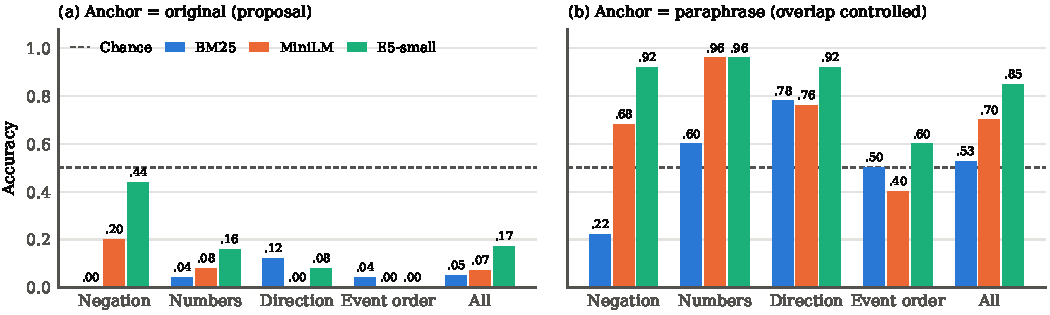
\includegraphics[width=\textwidth]{figures/contrast.pdf}
\caption{Meaning-change test (25 items per category; 95\% Wilson interval $\approx\pm0.19$).
(a) The edited sentence shares nearly all words with the anchor, and every system is fooled.
(b) With word overlap balanced, the encoders mostly detect negation and number changes, but
not event order. Direction items can be passed by word overlap alone (BM25 0.78).}
\label{fig:contrast}
\end{figure*}

\textbf{Keyword search is the strongest single system on synopsis queries
(Table~\ref{tab:main}).} We expected the opposite. On synopsis queries BM25 ranks the right report first 36\% of the
time, against 21\% for MiniLM and 19\% for E5 (all pairwise MRR differences $p<0.02$). We checked
whether exact identifiers explain this. Only 29\% of synopses repeat an identifier from their
narrative (an airport code, aircraft type or runway). These help every system, but BM25
still leads on the other 71\% (MRR@10 0.321 vs.\ 0.196). This agrees with the BEIR finding
that BM25 is a strong zero-shot baseline outside the encoders' training domain
\cite{thakur2021beir}. A likely factor is that ASRS text is full of abbreviations
(FL240, LNAV/VNAV, RA) that general-English encoders have rarely seen; aviation-specific
models such as Aviation-BERT \cite{chandra2023aviationbert} and SafeAeroBERT
\cite{andrade2023safeaerobert} target this gap, but we have not tested them. On topical
queries BM25 and MiniLM do not differ significantly (nDCG@10 0.630 vs.\ 0.591,
$p{=}0.29$).

\textbf{The two signals are complementary.} BM25+MiniLM fusion improves topical
nDCG@10 by 0.076 over BM25 ($p{=}0.0015$) and by 0.115 over MiniLM ($p<0.001$), and it
has the best Recall@100 on synopses in Table~\ref{tab:main}. It costs early precision there, though: it ranks the
target report first less often than BM25 alone (MRR@10 0.380 vs.\ 0.425, $p<0.001$). MiniLM beats BM25 on lenient P@10 (0.740 vs.\ 0.703)
but not on strict P@10 (0.463 vs.\ 0.537). It finds reports of the right event family
but often not the right mechanism. The best (BM25+MiniLM) and worst (E5) systems are the
same on the dev and test query halves; on the test half BM25 and MiniLM are level (0.548
vs.\ 0.543). Altitude queries, the proposal's
focus area, are the hardest for the encoders (nDCG@10: BM25 0.535, MiniLM 0.440, E5 0.159).

\textbf{E5 favours short texts, but that explains little of its gap.} E5 trails MiniLM on
retrieval despite being the newer retrieval model. Its similarity scores for short units
are \emph{lower} on average but 1.7 times as spread out (mean per-query z-score $-0.83$
for units under 30 words). That upper tail reaches the top: on topical queries, short units
fill 17.5\% of E5's top-10 results (MiniLM 7.3\%) but only 0.9\% of the index. These hits
are only slightly less relevant than E5's other top-10 hits (grade~2: 30\% vs.\ 36\%), so
even if they were as good as the rest, E5's P@10 would rise by about 0.01, against a gap
of 0.11 to MiniLM.

\begin{table}[t]
\centering
\caption{More encoders, ablations and the taxonomy graph. ``Whole'': one vector per
report, truncated at the input limit (MiniLM 256 tokens, cutting 59\% of reports; E5 512,
24\%). Graph oracle: upper bound. Contrast: overlap-controlled.}
\label{tab:ext}
\setlength{\tabcolsep}{3pt}
\begin{tabular}{@{}lcccc@{}}
\toprule
 & Synopsis & Topical & \multicolumn{2}{c}{Contrast}\\
\cmidrule(l){4-5}
System & MRR@10 & nDCG@10 & all & order\\
\midrule
BM25, whole report & \textbf{.458} & .621 & .53 & .50\\
BM25, keep negation      & .428 & .626 & .49 & .50\\
MiniLM, whole report & .271 & .615 & .70 & .40\\
E5-small, whole report & .255 & .410 & .85 & .60\\
\midrule
MPNet (110M)             & .257 & .622 & .85 & \textbf{.72}\\
BGE-small (33M)          & .287 & .610 & .85 & .60\\
BGE-base (110M)          & .308 & .583 & .82 & .56\\
BGE-large (335M)         & .336 & .623 & .88 & .64\\
E5-base (110M)           & .280 & .451 & .82 & .52\\
E5-large (335M)          & .299 & .556 & \textbf{.89} & .64\\
Qwen3 (0.6B), generic instr.  & .371 & \textbf{.746} & .86 & .48\\
Qwen3 (0.6B), aviation instr. & .303 & .728 & .86 & .48\\
\midrule
BM25+BGE-large (RRF)     & .419 & .680 & -- & --\\
BM25+Qwen3 (RRF)         & .446 & \textbf{.746} & -- & --\\
BM25 + graph (oracle)    & .435 (.643) & -- & -- & --\\
\bottomrule
\end{tabular}
\end{table}

\textbf{Larger encoders narrow the gap but do not close it (Table~\ref{tab:ext}).}
Synopsis MRR@10 rises with size in both families ($p<0.001$ small vs.\ large), and Qwen3 is the best encoder (0.371), yet all stay below BM25 (Qwen3
$-0.054$, $p<0.001$). Fused with BM25, Qwen3 is the first system to beat BM25 on chunks
(0.446 vs.\ 0.425, $p{=}0.018$; Recall@100 0.805 vs.\ 0.753) and ties it on whole reports
($p{=}0.23$). On topical queries Qwen3 beats BM25 (0.746 vs.\ 0.630, $p<0.001$) although
silver labels may favour lexical matches, while BGE-large, MPNet and BGE-small only tie it
($p\ge0.53$). E5's topical weakness shrinks with scale (E5-large $+0.105$ over E5-base,
$p<0.001$). Our aviation-specific instruction hurt Qwen3 on synopses (0.303 vs.\ 0.371 with
the generic one, $p<0.001$). We made both choices on validation data; the test split must
confirm them. Whole-report scoring changes no dense model
significantly on topical queries but helps BM25 on synopses (0.458, $p<0.001$), plausibly
because a synopsis summarises details from the whole narrative rather than from one
passage. For the encoders this ablation also truncates long reports, so it does not
isolate the effect of best-chunk scoring.

\textbf{The graph helps only as much as queries can be linked to it.} With oracle
linking it would raise synopsis MRR@10 from 0.425 to 0.643. The learned linker gets a synopsis's exact code set right for only 21\% of queries,
and the rerank gains 0.010 ($p{=}0.013$; whole reports $+0.012$, $p{=}0.002$). The topical
track cannot test the graph, as its silver labels come from the same codes. This fits Han
et al.\ \cite{han2025ragvsgraphrag}: graph retrieval wins on multi-hop questions, plain
retrieval on single-hop lookups like ours.

\textbf{Meaning-change test (Fig.~\ref{fig:contrast}).} In the proposal's condition, every
non-fusion system in Tables~\ref{tab:main}--\ref{tab:ext} prefers the one-word edit over
the true paraphrase (accuracy 5--35\%). Negation gains most from size (Qwen3 0.80,
BGE-large 0.68; smaller encoders 0.20--0.60). Surface
overlap dominates similarity for both keyword and embedding methods, so on this evidence
a small frozen encoder would rank ``descended'' above ``maintained altitude'' as a match
for ``did not descend''. With overlap controlled, the encoders do encode much of the meaning:
E5 0.85 and MiniLM 0.70 overall, with numbers at 0.96 for both (BM25 0.60). Direction
says less, since BM25 also passes 0.78 of it. Event order remains the weak spot (MiniLM
0.40, E5 0.60, both within the $\pm0.19$ interval around chance). Mean pooling alone does
not explain this: BGE-small, which uses the [CLS] token instead, also scores 0.60, and
scale does not help (BGE-large and E5-large 0.64, Qwen3 0.48).
BM25 scores 0.22 on negation. Keeping ``not'' in the index makes it worse (0.08), because
the paraphrases express negation with other words (``maintained altitude'').

\subsection{A pre-processing finding}\label{sec:prep-finding}
In our first run (v1, without placeholder removal or tail merging), 18.5\% of E5's top-10
matched passages on topical queries had fewer than 30 words, against 3.7\% of all chunks.
Many were placeholders such as ``[Narrative \#2 contains no additional information.]''.
Pre-processing v2 cut short units to 0.9\% of the index, yet their share of E5's top-10
barely fell (to 17.5\%) and its topical score barely moved (0.444 to 0.438). The short hits
are therefore mostly genuinely short reports, not artifacts.

\section{Future work}
\begin{enumerate}
\item \textbf{Human labels (next two weeks).} \texttt{asrsbench pool} merges the
top-10 of every system into blind, shuffled judging sheets (to be rebuilt with Qwen3). Both of us will judge with a
25\% overlap and report Cohen's $\kappa$, and we will extend the set toward the proposed
50--80 queries. Silver labels come from codes and synopsis keywords, so they may favour
lexical matches; the human labels will test that.
\item \textbf{Length bias.} E5's preference for short reports survived pre-processing
v2. Next we will test score calibration, which normalises each unit's score
against its typical similarity to queries, and fusion weights tuned on dev queries only.
\item \textbf{Stretch goals}: Qwen3-4B/8B and untruncated whole-report Qwen3 on a CUDA
GPU, a better query-to-code linker for the graph, and, in the proposal's order, report
versions (B), a small
fine-tune on near-miss pairs split by incident group (D), and ADS-B tracks (C).
\end{enumerate}
The synopsis test split is still unused and will be scored once, for the final report
(Nov.~30). The 20 topical test queries are already scored in Table~\ref{tab:main}, so the
queries we add for human labelling will serve as the held-out topical set. The talk on Nov.~23 will present the system comparison
and failure examples.

\bibliographystyle{IEEEtran}
\bibliography{references}

\end{document}
